\begin{figure}[htbp]
  \centering
  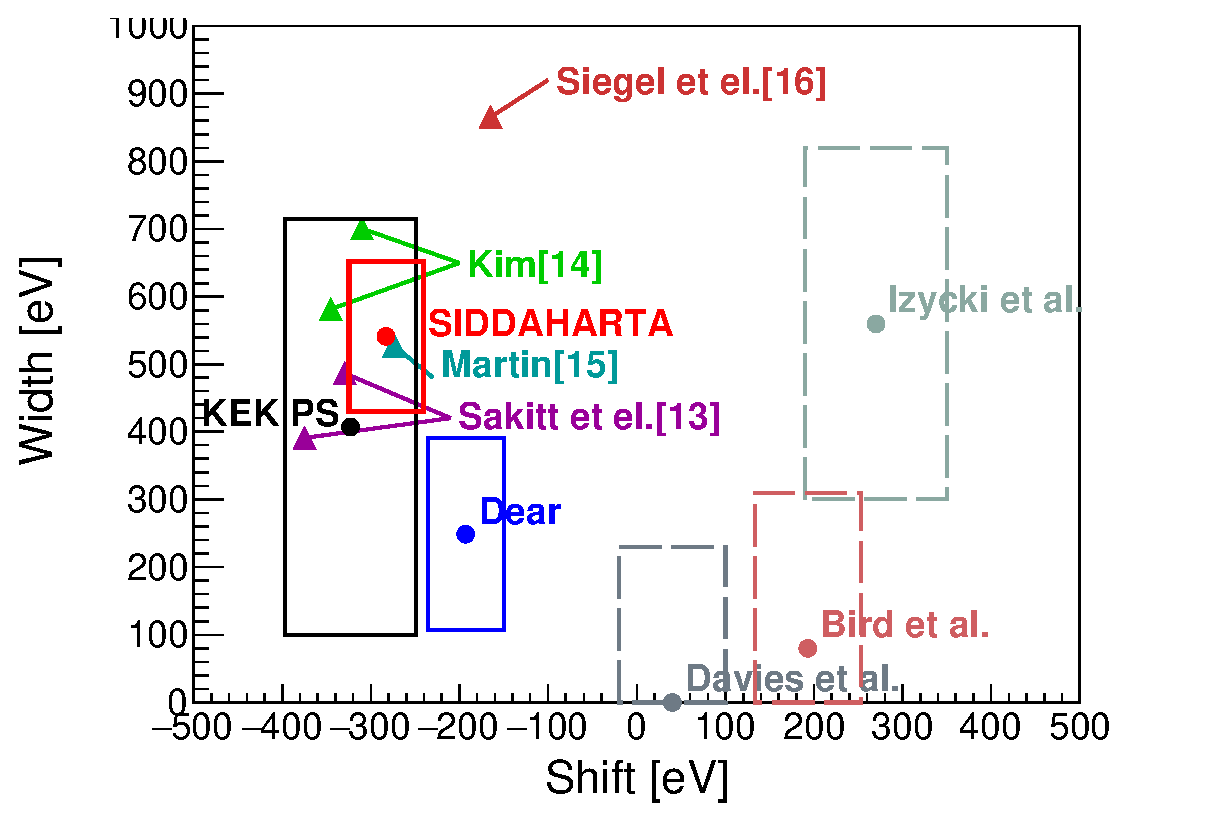
\includegraphics[width=12cm]{../pic/Dron/KN_int_map.eps}
  \caption{
    This figure is shown about the kaonic hydrogen.
    Triangle markers indicate theoretical calculations where $\bar{K}N$ scattering data were extrapolated to the $\bar{K}N$ threshold.
    Circle markers represent experimental values, and error ranges in the energy shift and width are indicated by squares.
    Dashed lines correspond to experiments using hydrogen gas targets conducted prior to 1990,
    while solid lines represent experiments conducted afterward.
  }
  \label{fig:KN_int}
\end{figure}


Considering the $\Lambda(1405)$ as a $\bar{K}N$ bound state, the $\bar{K}N$ interaction is expected to be attractive.
From the 1960's to the 1980's, various $K^-p \rightarrow$ meson-baryon, e.g., $K^- p$, $K^0 n$, $\pi \Lambda$, $\pi \Sigma$, and so on,
scattering data were measured on a hydrogen target using bubble chambers to study the $\bar{K}N$ interaction \cite{CERN1,CERN2,CERN3,CERN4,Gopal}.
This method of course did not allow access below the $\bar{K}N$ mass threshold and measurements in the low momentum region were difficult and data were insufficient.
Nevertheless,
the value of the $\bar{K}N$ interaction at the $\bar{K}N$ mass threshold was obtained by extrapolating it from the high momentum region,
where abundant data exist, using several models \cite{KN_int_1, KN_int_2, Martin, KN_int_3}.
These values are shown in Figure \ref{fig:KN_int} as the characteristic X-ray values for kaonic hydrogen, discussed below.
Due to the lack of data in the low momentum region, these values varied.
However, they were all attractive and consistent with the $\Lambda(1405)$ being a $\bar{K}N$ bound state.

An attempt to measure $\bar{K}N$ interactions at the $\bar{K}N$ mass threshold using kaonic hydrogen has been proposed.
In this method, a $K^-$ meson beam is stopped in a hydrogen target,
and the characteristic $X$-rays emitted when the kaon binds to a proton are utilized.
In the case of nucleon-meson, the characteristic $X$-ray is affected not only by electromagnetic interactions but also by the strong interactions
i.e. $\bar{K}N$ interaction,
leading to a shift in energy and a gain in width compared to the case where only electromagnetic interactions are present.
According to Deser-Trueman formula \cite{Deser, Deser2}, these shift and width are model-independent and given by
$\Delta E^{s}_{1}-\frac{i}{2}\Gamma_{1}=-2\alpha^3\mu_{c}^2a_{K^-p}$.
Where $\alpha$ is the fine structure constant, $\mu_{c}$ is the mass of the $K^-$-$p$ system,
and $a_{K^-p}$ is the scattering length of the $\bar{K}N$ interaction.
Several attempts were made in the 1980s using liquid hydrogen targets \cite{KaonicH_1, KaonicH_2, KaonicH_3}.,
but the results showed a positive energy shift, indicating that the $\bar{K}N$ interaction is repulsive,
contradicting $\bar{K}N$ scattering experiments.
To improve the poor signal-to-noise ratio of these experiments,
experiments were conducted at KEK PS using gaseous hydrogen targets, and a negative energy shift was reported,
thus confirming that the $\bar{K}N$ interaction is attractive \cite{KEK_E228}.

Once the $\bar{K}N$ scattering experiments and characteristic $X$-ray measurements were found to be qualitatively consistent,
this led to further investigations into the $\bar{K}N$ interaction.
The scattering length from characteristic $X$-ray measurements was determined more precisely by DEAR \cite{Dear} and the SIDDHARTA Collaboration \cite{SHIDDARTA}.
The values of these experiments are also shown in Figure \ref{fig:KN_int}.
The SIDDHARTA data serve as a crucial constraint on the $\bar{K}N$ mass threshold,
playing a key role in constraining the $\bar{K}N$ scattering amplitudes discussed later.
